\documentclass[../main]{subfiles}
\ifSubfilesClassLoaded{
    \dominitoc
    \tableofcontentsfile
    \pagenumbering{arabic}
    \setcounter{page}{1}
	\setcounter{chapter}{2}
	\addbibresource{../Biblio/biblio.bib}
}{}

\begin{document}
\chapter{Analyse du mécanisme de relaxation}\label{chap:relaxation}
\graphicspath{{./},{07-Relaxation/}}

\minitoc

\section{Introduction}

Le processus de relaxation que nous avons défini au chapitre précédent est une méthode originale de l'algorithme CxSOM permettant de construire des connexions bidirectionnelles entre cartes.
Afin de valider son utilisation en tant que méthode de recherche de BMU et d'interface entre cartes, nous présentons dans ce chapitre une étude expérimentale de ses propriétés de convergence.

\subsection{Origine du mécanisme de relaxation~: passage du calcul cellulaire au calcul à l'échelle d'une carte}

Le mécanisme de relaxation que nous proposons, qui s'appuie sur les calculs d'activations et le déplacement de BMU, hérite des architectures de cartes cellulaires développées précédemment dans l'équipe \cite{khouzam_neural_2014,menard05}.
Dans ces travaux, le processus dynamique d'apprentissage s'appuyait sur des champs neuronaux dynamiques couplés (DNF) comme pendant cellulaire de la recherche de BMU.
Les champs neuronaux dynamiques, introduits en \cite{Amari1977DynamicsOP} sont des systèmes dynamiques temporels modélisant à gros grains l'activité spatiotemporelle d'une population de neurones impulsionnels. 
Au lieu de s'intéresser à l'activité d'un seul neurone, tel que son taux de décharges, le modèle de DNF calcule un potentiel d'activation $u(x,t)$ sur un ensemble de positions continues $x$ au cours du temps $t$, réagissant à un stimulus d'entrée $s(x,t)$. Ce stimulus correspond à une réponse scalaire qui modélise la réponse spatio-temporelle des neurones à un stimulus externe.
Les positions $x$ s'étendent sur l'espace des caractéristiques du signal d'entrée et représentent une valeur dans cet espace. Ainsi, un DNF réagissant à un stimulus $s(x,t)$ 1D est en une dimension, etc.
L'évolution du potentiel $u$, pour un exemple en temps continu sur un espace $x$ en une dimension, s'exprime par l'équation différentielle~:

\begin{equation}\label{eq:DNF}
	\tau \frac{\partial u(x,t)}{\partial t} = - u(x,t) + s(x,t) + h + \int_{-\infty}^{\infty} \omega(x - y)g(u(y,t))dy 
\end{equation}

\begin{figure}
	\centering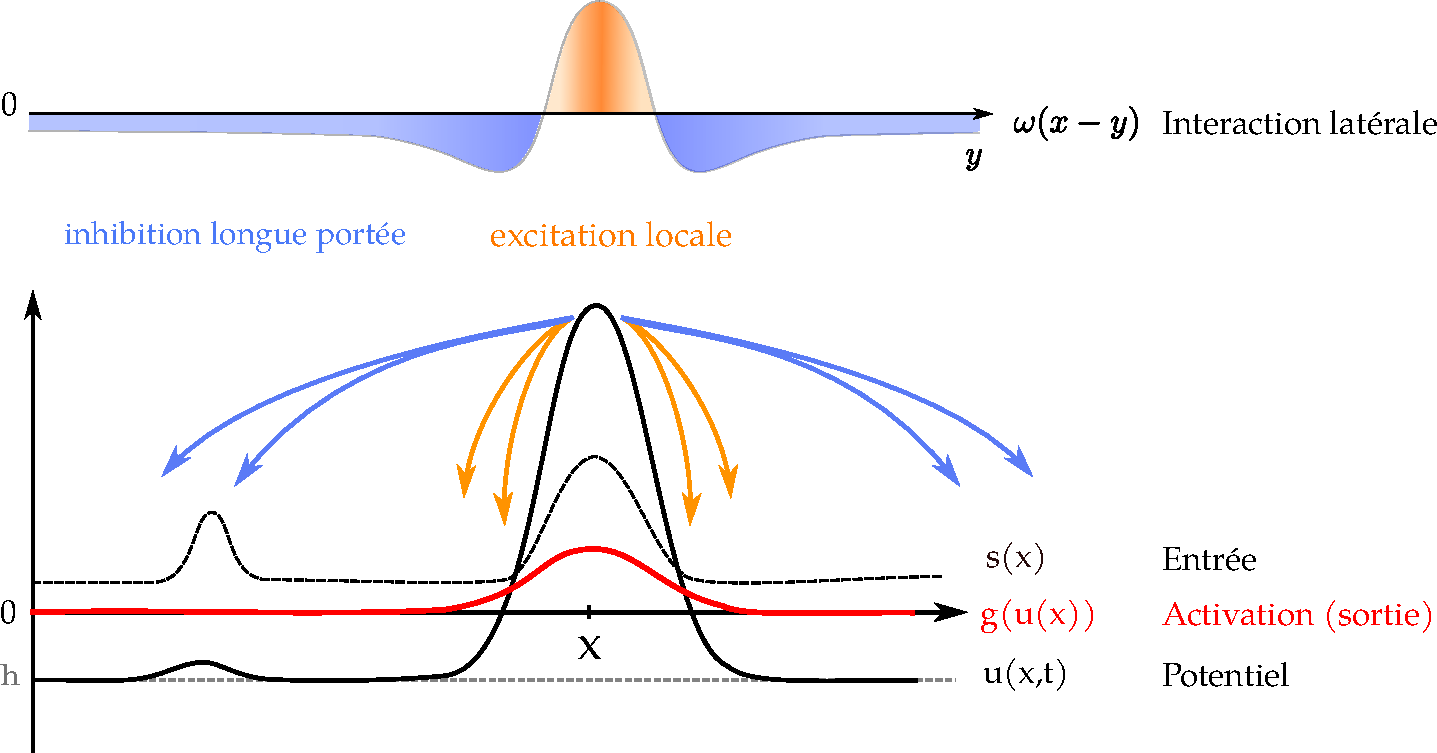
\includegraphics[width=0.9\textwidth]{DNF.pdf}
	\caption{Schéma des éléments intervenant dans le calcul du potentiel $u$ du DNF (équation~\ref{eq:DNF}), ici pour un signal d'entrée $s(x)$ constant dans le temps.
	Le potentiel $u$ du DNF évolue grâce aux interactions entre les positions $x$, grâce à l'activation de tout le DNF convolué par l'interaction latérale $\omega(x - y)$ en chaque $x $.
	L'évolution du DNF concentre toute l'activation $g(u(x,t))$ autour d'un seul point, qui se situe au maximum de $s(x)$~: le maximum local de gauche n'a pas de représentation dans l'activation totale, à cause des connexions inhibitrices.
	Cet exemple de DNF implémente ainsi un mécanisme de Winner-Take-All. En fonction des paramètres, les DNF peuvent présenter d'autres types de réponses. \label{fig:DNF}
	}
\end{figure}

Les éléments principaux du calcul de $u$ sont illustrés en figure~\ref{fig:DNF}.
$s(x,t)$ est le signal d'entrée du DNF, et $h$ est un niveau de repos.
Ensuite, l'évolution du potentiel en chaque point $x$ dépend de l'état d'activation de tout le DNF, grâce à l'intégration sur toutes les positions $y$ de l'activation.
Dans ce terme d'intégrale, $g(u(y))$ est une fonction sigmoïde centrée en zéro représentant l'activation du champ neuronal en une position $y$. Elle s'applique sur le potentiel $u(y)$, de telle sorte qu'une position $y$ du champ ne sera prise en compte dans l'interaction générale que si son potentiel dépasse un certain seuil d'activation. $g(u(x,t))$ correspondra également à la valeur utilisée comme sortie du DNF.
$\omega(x-y)$ (en haut de la figure) est un terme d'interaction latérale, en général une différence de gaussiennes, rendant le voisinage proche de $x$ \emph{excitateur}~: son activation renforce le potentiel $u(x,t)$, tandis que le voisinage à plus longue distance est inhibiteur.
En résumé, le calcul du potentiel $u(x,t)$ en tout point $x$ dépend de l'activation de l'ensemble des positions du DNF, convoluée par le terme d'interaction latérale.

Le calcul du potentiel $u(x,t)$ d'un DNF sur un stimulus d'entrée résulte en la formation de bulles d'activités évoluant dans les zones ou le signal d'entrée est élevé.
Les comportements du DNF varient en fonction des paramètres choisis~; une des applications possibles est l'implémentation d'un mécanisme de Winner-Take-All. 
Dans l'exemple présenté en figure~\ref{fig:DNF}, l'activation $g(u(x))$ du DNF évoluera pour former une seule bulle (en rouge) centrée en la valeur où $s(x)$ est maximal, sans représenter le maximum secondaire de $s$.
Par ailleurs, les calculs permettant le mécanisme Winner-Take-All implémenté par le DNF se rapprochent de calculs cellulaires~:~ils ne dépendent que d'un voisinage de chaque position.
En effet, même si l'évolution de $u(x,t)$ prend en compte en chaque point tout le champ d'activation, les positions qui ont vraiment une influence sont situées sur un voisinage de $x$, compte tenu de la forme du terme d'interaction latérale $w(x-y)$.


Des DNF peuvent réagir à plusieurs signaux d'entrée $s_i(x)$ et être couplés en des architectures dynamiques, exhibant des mécaniques complexes, présentées par exemple en \cite{Fix2011ADN, Sandamirskaya2014DynamicNF}.
Ces travaux montrent que ce couplage permet de générer des comportements autonomes au sein de structures de DNF, au lieu de la seule réaction à l'entrée $s$ engendrée par le DNF simple.
S'appuyant sur cet aspect dynamique et cellulaire, les architectures de cartes auto-organisatrices couplées en~\cite{khouzam_neural_2014,menard05} utilisent des DNF couplés associés aux différentes cartes. Leur évolution couplée, appelée relaxation dans ces travaux, amènent ces DNF à se stabiliser sur des bulles d'activité sur chaque carte, définissant les unités qui seront mise à jour.
Les architectures de cartes proposées dans ces travaux vont au delà de l'utilisation des DNF comme mécanismes d'attention et de sélection, puisque des mécanismes d'apprentissage dans les cartes sont modulés par l'activité résultante du DNF. Cette activité joue le même rôle que la fonction de voisinage d'une SOM.
Les DNF implémentent ainsi un calcul cellulaire manquant aux cartes auto-organisatrices classiques pour réaliser des calculs au niveau du neurone et non de la carte.
Cependant, l'optimisation des paramètres du DNF est délicate à réaliser \cite{fix:hal-00869726}, et le calcul du potentiel est extrêmement gourmand en ressources.
Les cartes de Kohonen classiques ont simplifié le processus de calcul de champs neuronaux par une recherche de BMU par activation. Ce calcul implémente, comme les DNF, un mécanisme de Winner-Take-All, mais est centralisé à l'échelle de la carte.
Dans le même esprit que l'utilisation d'une activation chez Kohonen pour trouver le BMU au lieu d'un mécanisme cellulaire, le mécanisme de relaxation que nous avons proposé dans CxSOM cherche à conserver ce processus dynamique de recherche de BMU menant à un consensus global, mais en plaçant les calculs à l'échelle d'une carte. 
% Le choix d'un BMU $\bmu$ dans une carte auto-organisatrice par un $\argmax$ équivaut à la génération d'une bulle d'activité centrée en $\bmu$ dans un DNF. 
% Le processus dynamique de relaxation que nous utilisons suit le même principe, en passant des mécanismes cellulaires réalisés dans les DNF couplés vers des calculs d'activité et de BMU. Le couplage entre les activités des cartes reste par contre un processus dynamique.
Ce choix simplifie les calculs réalisés au sein d'une carte et permet d'envisager l'étude de grandes architectures de cartes, tout en conservant une proximité avec une vision cellulaire des cartes auto-organisatrices.

Dans notre modèle, le mécanisme de relaxation possède deux fonctions. Il permet de trouver un BMU dans chaque carte, c'est-à-dire une position que les poids utiliseront pour leur mise à jour pendant l'apprentissage. En même temps, il joue le rôle d'interface entre les cartes.

\subsection{Problématique du chapitre}

Dans ce chapitre, nous explorons la validité de la relaxation en tant que mécanisme d'interface entre cartes et de recherche de BMU.
Nous proposons d'abord une formalisation plus détaillée qu'au chapitre \ref{chap:modele} de l'algorithme de relaxation, qui permettra de mettre en valeur les éléments intervenant dans la dynamique de la relaxation. Nous formulerons ainsi la relaxation sous forme d'une recherche de maximum global à l'architecture, soit une extension de la recherche d'argmax dans une SOM classique.
Cette formalisation de l'algorithme nous permettra de proposer des conditions de convergence que la relaxation doit satisfaire afin de pouvoir être considérée comme une recherche de \og Best Matching Unit \fg{}, ayant un sens pour la mise à jour des poids des cartes.

Nous chercherons ensuite à vérifier ou invalider ces conditions de convergence sur des exemples.
Le comportement de la relaxation dépend complètement des configurations des poids externes et contextuels des cartes de l'architecture, qui résultent d'un processus de mise à jour et n'ont pas de formulation analytique. Sans chercher à apporter une preuve de convergence, ce chapitre propose des hypothèses et intuitions à partir d'exemples. Pour cela, nous visualiserons et caractériserons des trajectoires de relaxation sur des exemples de configuration de poids, à différents instants de l'apprentissage.


\section{Formalisation de l'algorithme de relaxation}

Dans cette section, nous formulons l'évolution de la relaxation comme une suite récurrente, ainsi que le problème d'optimisation auquel elle cherche à répondre.
Nous introduisons ainsi des notations plus détaillées qui nous permettront d'observer les quantités relatives à l'évolution de la relaxation en section suivante.

\subsection{Formulation de l'évolution des BMUs lors de la relaxation}\label{sec:formulation_suite}

La relaxation est une suite de positions dans l'espace des positions des $n$ cartes, notée $(\mathbf{\bmu})_\tau = (\bmu\m{1}_\tau,\cdots,\bmu\m{n}_\tau)$. Nous voulons exprimer ici son équation d'évolution. Il s'agit de la suite des positions des \og BMU temporaires \fg{}, utilisés comme entrées contextuelles au long de la relaxation.

Définissons d'abord la suite $(\mathbf{\hat{p}})_\tau = (\hat{p}\m{1}_\tau, \cdots, \hat{p}\m{n})$, qui correspond à la position maximisant l'activité globale de chaque carte $i$ à l'instant $\tau$~:
\begin{equation}
\begin{gathered}
\forall i, \: \hat{p}\m{i}_{\tau} = \argmax\limits_p(a_g\m{i}(p, \inpx\m{i}, \bmu\m{i_0}_\tau, \cdots \bmu\m{i_K}_\tau))\\
 i_0, \cdots i_K \: \text{indices des cartes nourrissant la carte $i$}.
\end{gathered}
\label{eq:pstar}
\end{equation}

L'équation d'évolution de la suite $(\mathbf{\bmu})_\tau$ s'écrit alors à partir de $\hat{p}_\tau$~:

\begin{equation}
\forall i, \: \bmu\m{i}_{\tau+1} = 
\begin{cases}
\bmu\m{i}_{\tau} + sgn(\hat{p}\m{i}_{\tau} - \bmu\m{i}_{\tau}) \times \Delta \; & \text{si $\lvert \hat{p}\m{i}_{\tau} - \bmu\m{i}_{\tau}\rvert > \Delta$ } \\
\hat{p}\m{i}_{\tau} \; \text{sinon}	
\end{cases}
\label{eq:evolution}
\end{equation}

$sgn$ est la fonction signe.
$a_g\m{i}$ est une fonction des poids $\w\ext\m{i}, \w\cont\m{i}$ de la carte, de son entrée externe $\inpx\m{i}$ et des entrées contextuelles.
Lors du processus de relaxation, les poids et l'entrée $\inpx\m{i}$ restent constants. 
Le calcul de $a_g\m{i}$ à l'instant $\tau$ ne dépend donc pas de $\tau$.

Finalement, pour toute carte $i$, $\hat{p}\m{i}_{\tau}$ dépend uniquement de $(\bmu\m{i_0}_\tau, \cdots \bmu\m{i_K}_\tau)$ lors du processus de relaxation.
En posant $f\m{i}$ toute la partie droite de l'équation \ref{eq:evolution}, on peut donc écrire~:

\begin{equation}
\forall i, \; \bmu\m{i}_{\tau +1} = f\m{i}(\bmu\m{1}_\tau,\cdots,\bmu\m{n}_\tau)
\label{eq:fonction}
\end{equation}

Soit, pour l'ensemble des composantes: 
\begin{equation}\label{eq:f}
\mathbf{\bmu}_{\tau+1} = \mathbf{f}(\mathbf{\bmu}_\tau)
\end{equation}
$\mathbf{f} = (f\m{1}, \cdots, f\m{n})$ dépend des configurations de poids de toutes les cartes et des entrées externes.

Si $(\mathbf{\bmu})_\tau$ converge, alors elle converge vers un point fixe de la fonction $\mathbf{f}$, soit une position $\mathbf{\bmu}$ vérifiant~:
\begin{equation}
\mathbf{\bmu} = \mathbf{f}(\mathbf{\bmu})
\label{eq:suite}
\end{equation}

C'est-à-dire, d'après \ref{eq:evolution}, les points vérifiant $$\forall i, \: \bmu\m{i} = \argmax\limits_p a_g\m{i}(p, \inpx\m{i}, \bmu\m{1}, \cdots, \bmu\m{n})$$

Rien ne garantit que des points fixes existent ni que la suite converge~: $\mathbf{f}$ dépend de l'organisation des poids externes et contextuels de chaque carte, qui sont aléatoirement répartis au début de l'apprentissage.
Pour des poids $\w$ quelconques, il n'existe généralement pas de point fixe.
Enfin, l'évolution de la suite $(\mathbf{\bmu})_{\tau}$ dépend de son initialisation.
Lors de l'apprentissage du modèle, nous prenons comme état initial une position $(\bmu\m{1}_0, \cdots , \bmu\m{n}_0)$  telle que~: 
\begin{equation}
\begin{cases}
\bmu\m{1}_0 = \argmax\limits_p a_e\m{i}(p,\inpx\m{1})\\
\cdots \\
\bmu\m{n}_0 = \argmax\limits_p a_e\m{i}(p,\inpx\m{n})\\
\end{cases}
\label{eq:init}
\end{equation}

Nous nous intéresserons plus généralement dans ce chapitre à l'évolution de relaxation pour $(\bmu\m{1}_0, \cdots , \bmu\m{n}_0)$ quelconques.

Cette expression de la relaxation met en évidence le fait que la recherche de BMU est une trajectoire dans l'espace $(p\m{1}, \cdots, p\m{n})$. Les valeurs du champ $\mathbf{f}(p\m{1}, \cdots, p\m{n})$ sont constantes selon $\tau$ au cours de la relaxation. Pour une architecture de deux cartes, nous pouvons facilement calculer cette fonction $\mathbf{f}$ en tout point $(p\m{1}, p\m{2})$ et en chercher les points fixes par une recherche exhaustive. 
La relaxation est une trajectoire dans l'espace des arguments de $\mathbf{f}$, qui pourra être représentée facilement dans le cas de deux cartes.
C'est ce que nous ferons en section~\ref{sec:relax_expe}.
La recherche des points fixes de la fonction $\mathbf{f}$ nous permettra de vérifier leur existence et le tracé des trajectoires nous permettra d'observer comment la relaxation converge vers ces points.

\subsection{Formulation du problème d'optimisation}\label{sec:formulation_argmax}

La relaxation que nous venons de décrire est la recherche d'un ensemble de valeurs $\mathbf{\bmu} = (\bmu\m{1}, \cdots, \bmu\m{n})$ par une heuristique de recherche d'un point maximisant l'activité dans chaque carte. Il s'agit de l'extension à CxSOM du calcul d'argmax, définissant le BMU, réalisé dans une SOM classique. 
Nous avons exprimé les trajectoires selon $\tau$~; nous voulons également interpréter la relaxation comme la recherche d'un maximum dans l'activité globale de l'architecture de cartes, que nous détaillons ici. 

Rappelons les équations de calcul d'activation~:
dans chaque carte $i$, l'activité globale est définie par~:
\begin{equation}\label{eq:ag}
	a_g\m{i}(p, \inpx\m{i}, \inpc\m{i}_0, \cdots, \inpc\m{i}_K) = \sqrt{a_e\m{i}(p,\inpx\m{i})(\frac{1}{2}a_e\m{i}(p,\inpx\m{i}) + \frac{1}{2}a_c\m{i}(p,\inpc\m{i}_0, \cdots, \inpc\m{i}_K))}
\end{equation}
Avec $(\inpc\m{i}_0, \cdots, \inpc\m{i}_K)$ les $K$ entrées contextuelles de la carte. Lors de la relaxation, elles correspondent aux valeurs $\bmu\m{i_k}_\tau$.

L'activité contextuelle $a_c\m{i}$ d'une carte est définie comme la moyenne des activités contextuelles sur chaque couche de poids contextuels~:
\begin{equation}
	a_c\m{i}(p,  \inpx\m{i}, \inpc\m{i}_0, \cdots, \inpc\m{i}_K) = \frac{1}{K+1}\sum_{k=0}^{K}{a_{ck}\m{i}(p, \inpc\m{i}_k)}
\end{equation}

Pour simplifier les notations, nous noterons que les entrées contextuelles d'une carte $i$ sont $\{ \inpc\m{i}_k, k = 0 \cdots n , k \neq i  \}$.
Par la relaxation, nous cherchons une position $(\bmu\m{1}, \cdots, \bmu\m{n})$ telle que pour tout $i$, $a_g\m{i}(p,  \inpx\m{i}, \inpc\m{i}_0, \cdots, \inpc\m{i}_K)$ soit maximale. $a_g\m{i}$ est à valeurs positives pour tout $i$~; maximiser individuellement $a_g\m{i}$ revient à maximiser leur somme.

Nous proposons d'exprimer la relaxation comme une heuristique de recherche d'une solution du problème d'optimisation suivant~:
\begin{equation}\label{eq:opti}
	\begin{cases}
	\maximise\limits_{\bmu\m{1}, \cdots, \bmu\m{n}}\;& \sum_{i = 1}^n a_g\m{i}(\bmu\m{i},\inpx\m{i},\inpc_0\m{i}, \cdots, \inpc_n\m{i}) \\
	\text{Sous Contrainte}\; &\forall i,\:\forall k \neq i, \; \inpc_k\m{i} = \argmax\limits_p a_g\m{k}(p, \inpx\m{k}, \inpc_0\m{k}, \cdots, \inpc_n\m{k})
	\end{cases}
\end{equation}


En effet, par définition de l'argmax, toute solution du problème~\ref{eq:opti} vérifie~:
$$\forall i, \: \bmu\m{i} = \argmax\limits_p a_g\m{i}(p, \inpx\m{i}, \bmu\m{1}, \cdots, \bmu\m{n})$$
Il s'agit d'un point fixe de la fonction $\mathbf{f}$ définie en équation~\ref{eq:f}.
Cependant, cette fonction peut admettre plusieurs points fixes, qui sont dans ce cas des maximums locaux. 

Nous pouvons conclure de cette formulation que si $\mathbf{f}$ admet un unique point fixe et que la relaxation converge, alors $(\mathbf{\bmu})_\tau$ converge vers l'unique solution du problème d'optimisation~\ref{eq:opti}, qui maximise la somme des activités globales dans l'architecture.
Nous notons également d'après cette formulation que si un tel point fixe n'existe pas, la relaxation ne permet pas de trouver une solution approchée du problème d'optimisation~\ref{eq:opti}~: elle ne convergera simplement pas.

Nous nous interrogeons maintenant sur la nécessité de remplir les deux conditions d'unicité du point fixe et de convergence, afin de caractériser les propriétés qu'on attend effectivement du BMU.

\subsection{La relaxation permet-elle de trouver une \og \emph{Best Matching Unit} \fg{} ?}

\`A partir de l'équation~\ref{eq:opti}, nous nous interrogeons sur les conditions qui nous permettent de définir la valeur finale du processus de relaxation comme une \og Best Matching Unit \fg{} ayant un sens pour les règles de mise à jour des cartes.

Nous avons exprimé la valeur de convergence de la relaxation comme un point maximisant l'activité globale dans chacune des cartes. Nous attendons donc de la relaxation qu'elle converge pour pouvoir l'interpréter comme une recherche de BMU. 
Bien que nous ayons fixé une limite maximale d'itérations $\tau_{max}$, la valeur trouvée à l'issue de $\tau_{max}$ itérations sans convergence ne peut être interprétée comme un maximum d'activité, même local, et donc n'a pas de sens pour l'apprentissage. Nous avons également vu, en formalisant les équations d'évolution de la relaxation, que la convergence n'est pas assurée par les règles d'évolution, et qu'elle dépend au contraire des configurations de poids et des entrées.
Pour y répondre, nous présentons une évaluation expérimentale de la convergence du processus de relaxation, réalisée sur des cartes 1D et 2D prenant des entrées externes 1D.
Cette évaluation  sera réalisée en section~\ref{sec:relax_conv} sur des exemples d'apprentissage d'une architecture de deux et trois cartes, qui sont les architectures auxquelles nous nous sommes principalement intéressée lors de cette thèse.


Ensuite, la notion de Best Matching Unit est définie au sein d'une carte de Kohonen classique comme l'unité possédant l'activité maximale pour une entrée fixée. Cette activité dépend de l'entrée et des poids de la carte.
Pour parler d'un algorithme de recherche du BMU, on attend donc que la position trouvée soit relative uniquement aux poids de la carte et aux entrées externes de l'architecture~: elle ne doit pas dépendre de l'initialisation du processus de relaxation.
Dans ce sens, nous chercherons en second lieu à observer si la valeur trouvée à l'issue de la relaxation, soit le point de convergence s'il existe, ne dépend pas des conditions initiales de la relaxation.
Cette propriété marquera le fait que le BMU est relatif à seulement l'entrée et l'état des poids de la carte et aura donc un sens pour l'apprentissage.
En section~\ref{sec:relax_expe} nous étudierons empiriquement si la fonction $\mathbf{f}$ générant la suite $\mathbf{\bmu}_\tau$ admet un point fixe, et si la suite converge vers ce point indépendamment des valeurs d'initialisation.

\section{\'Etude expérimentale de la convergence de la relaxation}\label{sec:relax_conv}

Nous nous intéressons à la convergence de la relaxation au cours d'un processus d'apprentissage complet d'architectures de deux et trois cartes. 
Les entrées $\inpx\m{1}$ et $\inpx\m{2}$ que nous présentons à chaque carte sont les coordonnées $x$ et $y$ de points situés sur un cercle de centre 0.5 et de rayon 0.5, cf. figure~\ref{fig:input_3som} p.~\pageref{fig:input_3som}. La disposition des entrées a peu d'importance ici, et nous détaillerons ce choix de disposition dans les chapitres suivants~; notons simplement que les entrées de chaque carte sont normalisées, et chacune s'étend sur toutes les valeurs entre 0 et 1.
Pendant l'apprentissage, nous effectuons des phases de test à des temps réguliers $t$, à poids figés, sur 5000 points tirés selon la mêmes distribution d'entrée. 
Nous comptons ensuite, pour chaque entrée de test réalisé au temps $t$, le nombre de pas nécessaires avant la convergence de la relaxation. Lors de ces tests, nous avons initialisé la relaxation à la position $\mathbf{\bmu}_0$ maximisant l'activité externe de chaque carte.

En pratique, l'algorithme de relaxation s'arrête si la relaxation dépasse $\tau_{max}$ ici fixé à $1000$ itérations~; nous considérerons que la relaxation n'a pas atteint un point de convergence lors d'une itération de test si le nombre de pas de relaxation a atteint $\tau_{max}$.
\`A partir de ces valeurs, nous traçons l'évolution du nombre de pas moyens nécessaires à la convergence au cours de chaque phase de test $t$.
Nous traçons également le taux de convergence~: il s'agit de la proportion d'entrées, sur les 5000 entrées d'un même test au temps $t$, pour lesquelles la relaxation a convergé.
Ces deux valeurs sont tracées en figure~\ref{fig:conv_evolution}. Il s'agit de la moyenne et de l'écart type du nombre moyen de pas de relaxation et du taux de convergence, obtenus sur 10 répétions d'une même expérience, sur des architectures de deux cartes (en bleu) et trois cartes (en orange).
La figure~\ref{fig:conv_evolution2D} présente ces valeurs sur des expériences réalisées avec des cartes 2D, prenant les mêmes entrées 1D que l'architecture de cartes 1D.

\begin{figure}
	\centering
	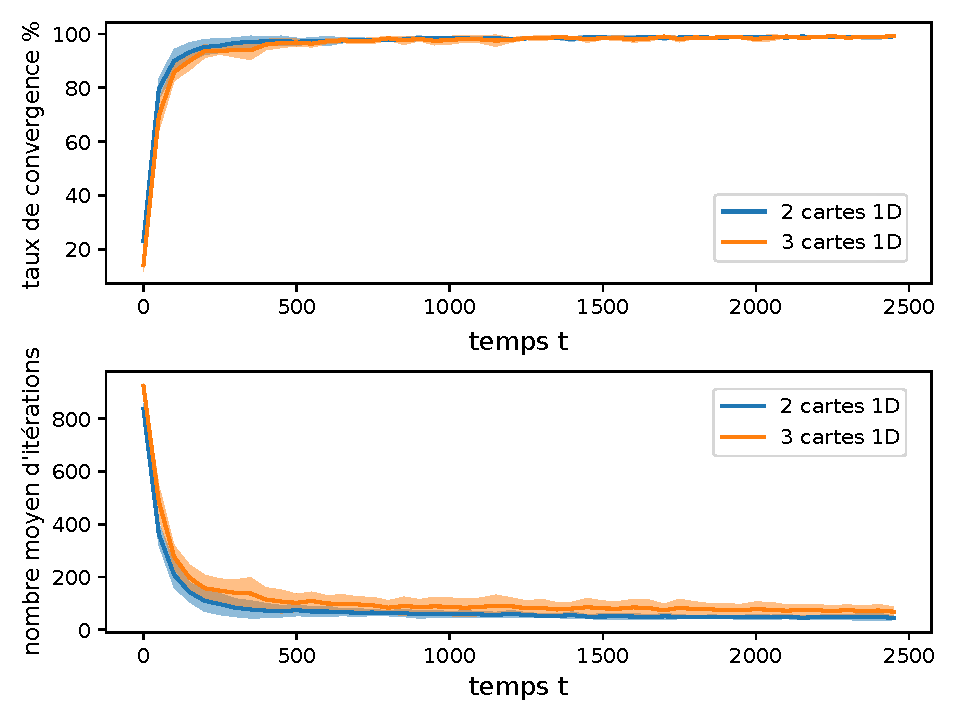
\includegraphics[width=0.7\textwidth]{1D_conv_evolution_total_french.pdf}
	\caption{En haut: évolution de la moyenne et l'écart-type du taux de convergence de la relaxation au cours de l'apprentissage, sur deux et trois cartes 1D. En bas~: évolution du nombre moyen de pas nécessaires à la convergence de la relaxation. Nous observons qu'au début de l'apprentissage, la relaxation converge rarement. La relaxation converge dans plus de 95\% des cas en fin d'apprentissage~: le BMU trouvé est alors une position stable maximisant les activités de chaque carte. Cette position a bien un sens de \og Best Matching Unit \fg{} pour l'apprentissage.
	Les tracés représentent les moyennes et l'écart-type des valeurs sur 10 expériences. \label{fig:conv_evolution}}
	\end{figure}

\begin{figure}
	\centering
	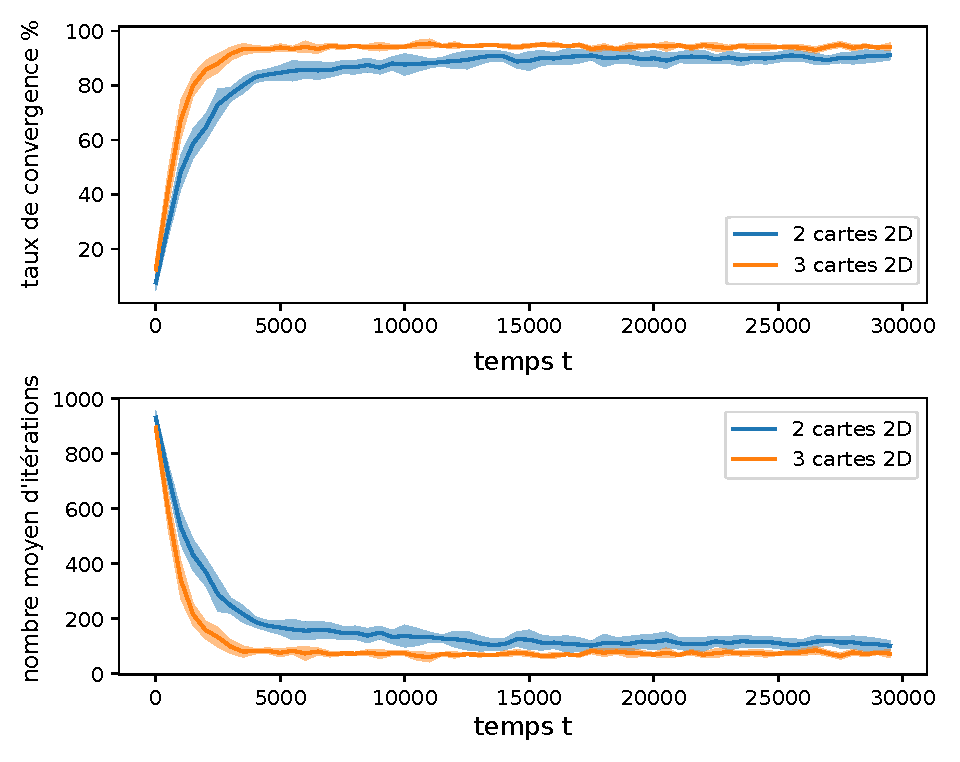
\includegraphics[width=0.7\textwidth]{2D_conv_evolution_total_french.pdf}
	\caption{En haut: évolution de la moyenne et l'écart-type sur 10 apprentissages du taux de convergence de la relaxation, sur deux et trois cartes 2D. 
	Comme pour des cartes 1D, la relaxation converge bien en fin d'apprentissage, indiquant que le BMU trouvé par la relaxation a un sens. La relaxation converge rarement au début de l'apprentissage.}
	\label{fig:conv_evolution2D}
	\end{figure}

Plusieurs situations peuvent se traduire par une non-convergence de la relaxation dans notre cadre expérimental~:
\begin{itemize}
\item La relaxation évolue vers un point fixe, mais trop lentement pour y arriver en moins de $\tau_{max} = 1000$ itérations.
\item La relaxation évolue vers un cycle limite, composé d'un nombre réduit d'unités se succédant alternativement comme $\mathbf{\bmu_\tau}$ lors de la relaxation.
\item La relaxation évolue sans répétition d'un motif dans chaque carte~: il s'agit d'une évolution chaotique.
\end{itemize}

Nous évitons le premier cas en fixant la limite $\tau_{max}$ assez grande par rapport à la taille de la carte~: les cartes sont de taille 500 et le pas d'évolution de la relaxation d'une dizaine d'unités.
La convergence, si elle existe, est rapide. Les cas de non-convergence concernent la deuxième et la troisième situation. 
Nous observerons plus précisément les trajectoires dans la section suivante~; on s'intéresse ici seulement à la question de la convergence.

Les figures~\ref{fig:conv_evolution} et \ref{fig:conv_evolution2D} montrent qu'au début de l'apprentissage, lorsque les poids sont initialisés aléatoirement, la relaxation atteint un point de convergence dans seulement 20\% des cas. Lorsque les cartes sont bien dépliées en fin d'apprentissage, la relaxation évolue vers un point de convergence dans plus de $95\%$ des cas pour des cartes 1D, et $90\%$ pour des cartes 2D. L'évolution de la convergence est similaire pour des architectures de deux et trois cartes.

D'une part, ces observations montrent que le BMU a un sens en fin d'apprentissage~: lorsque la relaxation a convergé, $\mathbf{\bmu}$ représente bien une position correspondant au maximum de l'activité de chaque carte.
D'autre part, nous avions remarqué d'après la formulation de la relaxation section~\ref{sec:formulation_suite} que la convergence est loin d'être assurée lorsque les dispositions de poids sont quelconques, ce qui est  le cas en début d'apprentissage. 
Les observations confirment cette hypothèse~: la relaxation converge seulement dans 20 \% des cas au début de l'apprentissage, lorsque les poids ne présentent aucune forme de continuité ou d'organisation.
Toutefois, le fait que la relaxation converge peu en début d'apprentissage ne perturbe pas l'organisation des poids, car nous avons pu observer dans la suite de nos expériences que les poids des cartes évoluent vers des états organisés et stables.

Cette propriété pourrait s'expliquer par le fait que le calcul de l'activité globale de la carte dépend principalement de l'activité externe, constante au cours de la relaxation, et que la relaxation est initialisée à une position correspondant au maximum de l'activité externe.
Bien que le BMU n'ait pas de sens en terme de maximum d'activité globale dans la plupart des cas au début de l'apprentissage, il apparaît rester dans des régions dont les poids externes sont proches de l'entrée externe.
Les poids externes vont alors se déplier correctement sur les entrées externes. Ce dépliement est par ailleurs plus rapide que celui des poids contextuels, car le rayon de voisinage externe est plus grand que le rayon de voisinage contextuel.
Une fois les poids externes dépliés, la relaxation semble converger. Le dépliement des poids contextuels, plus lent, s'effectuera donc sur des BMUs ayant un sens de maximum d'activité globale.

\section{Représentations des trajectoires de relaxation dans une architecture de deux cartes}

Nous avons observé que la relaxation converge en fin d'apprentissage dans la plupart des cas, mais ne converge que rarement en début d'apprentissage.
Nous étudions dans cette partie l'évolution de plusieurs processus de relaxation lancés sur des poids de cartes dans une même disposition, à présent en fixant l'entrée externe et en prenant des valeurs d'initialisation de relaxation $\mathbf{\bmu}_0$ différentes.
Dans le cas où la relaxation converge, nous voulons vérifier que le point de convergence ne dépend pas de l'initialisation de $\mathbf{\bmu}$.
Dans le cas où la relaxation ne converge pas, nous cherchons à observer les trajectoires menant à ces cas de non-convergence. Cette étude concerne des architectures de deux cartes 1D.

\subsection{Méthode de représentation\label{sec:relax_expe}}

% Cette partie présente des résultats sur deux exemples de configurations de poids. 
% Nous avons réalisé ces observations sur d'autres configurations de poids et d'entrées, qui nous permettent d'être plus générale sur les conclusions que nous présentons, mais cette étude reste empirique. Nos conclusions sont donc à voir comme des observations.
Reprenons les notations de la section~\ref{sec:formulation_suite}, appliquées à une architecture de deux cartes 1D. La suite des maxima d'activation au cours de la relaxation s'écrit~:
\begin{equation*}
	\begin{cases}
	\hat{p}\m{1}_\tau = \argmax\limits_p(a_g\m{1}(p, \bmu\m{2}_\tau))\\
	\hat{p}\m{2}_\tau = \argmax\limits_p(a_g\m{2}(p, \bmu\m{1}_\tau)) \\
	\end{cases}
	\end{equation*}
La suite des BMUs temporaires utilisés en entrées contextuelles des autres cartes est ensuite définie par~:
\begin{align*}
	&\begin{cases}
	\bmu\m{1}_{\tau+1} = \bmu\m{1}_\tau \pm \min(\lvert \hat{p}\m{1}_\tau - \bmu\m{1}_\tau \rvert, \Delta)  \\
	\bmu\m{2}_{\tau+1} = \bmu\m{2}_\tau \pm \min(\lvert \hat{p}\m{2}_\tau - \bmu\m{2}_\tau \rvert, \Delta) \\
	\end{cases}
	\end{align*}
Ici $\pm$ représente la direction de déplacement des $\bmu_\tau$ et correspond au signe de $\hat{p}\m{i}_\tau - \bmu\m{i}_\tau$ (voir l'équation \ref{eq:evolution}).


$\hat{p}\m{1}$ dépend seulement de l'entrée contextuelle $\gamma\{1}$, c'est-à-dire une position $p\m{2} \in [0,1]$, et inversement.
Les points de convergence possibles pour la relaxation sont les points fixes de $\mathbf{f}$ définie en \ref{sec:formulation_suite}. Il s'agit des valeurs pour lesquels $p\m{1} = \hat{p}\m{1}$ et $p\m{2} = \hat{p}\m{2}$, soit les valeurs nulles du champ~:
\begin{equation} 
	\mathbf{g}:\: (p\m{1}, p\m{2}) \rightarrow (\lvert \hat{p}\m{1} - p\m{1} \rvert,  \lvert \hat{p}\m{2} - p\m{2} \rvert)
\end{equation}

Sur les figures, nous traçons alors~:

\begin{itemize}
\item Les champs $\lvert \hat{p}\m{1} - p\m{1} \rvert$ en fonction de $(p\m{1}, p\m{2})$ et $\lvert \hat{p}\m{2} - p\m{2} \rvert$ en fonction de $(p\m{1}, p\m{2})$ afin de mettre en évidence les points de convergence possibles de la relaxation. 
\item Les valeurs $\mathbf{\bmu}_\tau$ sont des valeurs de l'espace des arguments $(p\m{1}, p\m{2})$ de $\mathbf{g}$. Nous tracerons sur la même figure que les champs les trajectoires de $\mathbf{\bmu}_\tau$ pour 200 valeurs d'initialisation différentes $\mathbf{\bmu}_0$, pour une même entrée $(\inpx\m{1}, \inpx\m{2})$. Si ces trajectoires convergent, elle le feront vers un zéro de $\mathbf{g}$~; nous chercherons ici à observer si elles convergent vers un même point.
\item Enfin, nous tracerons les champs correspondant au déplacement à effectuer de $(\bmu\m{1},\bmu\m{2})$ en tout point de l'espace. Ils s'agit des couples $(\pm \min(\hat{p}\m{1}_\tau - \bmu\m{1}_\tau, \Delta), \pm \min(\hat{p}\m{2}_\tau - \bmu\m{2}_\tau, \Delta)$. Nous tracerons également, sur ce champ de déplacements, les trajectoires des $\mathbf{\bmu}_\tau$ suivies lors de la relaxation.
\end{itemize}

\`A partir de ces représentations, nous voulons comparer l'évolution de la relaxation en début et à la fin d'un apprentissage. 
Nous avons vu en section~\ref{sec:relax_conv} qu'au début de l'apprentissage, la relaxation ne converge pas. Nous observerons alors quelles sont les trajectoires de relaxation dans ce cas.
En fin d'apprentissage, nous avons observé que la relaxation converge dans la majorité des cas~; nous chercherons à observer sur des exemples s'il existe un unique point de convergence, en fonction des conditions initiales de la relaxation.

\subsection{\'Evolution de la relaxation en début d'apprentissage}

\begin{figure}
	\begin{minipage}{0.5\textwidth}
	\centering
	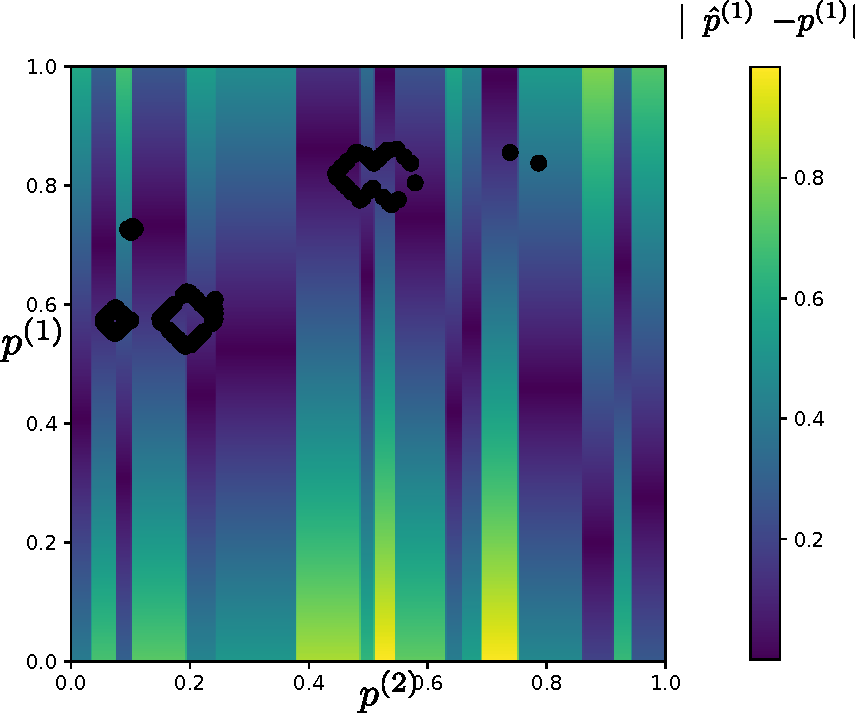
\includegraphics[width=\textwidth]{champ_X_006_t1_notraj.pdf}
	\end{minipage}
	\begin{minipage}{0.5\textwidth}
	\centering
	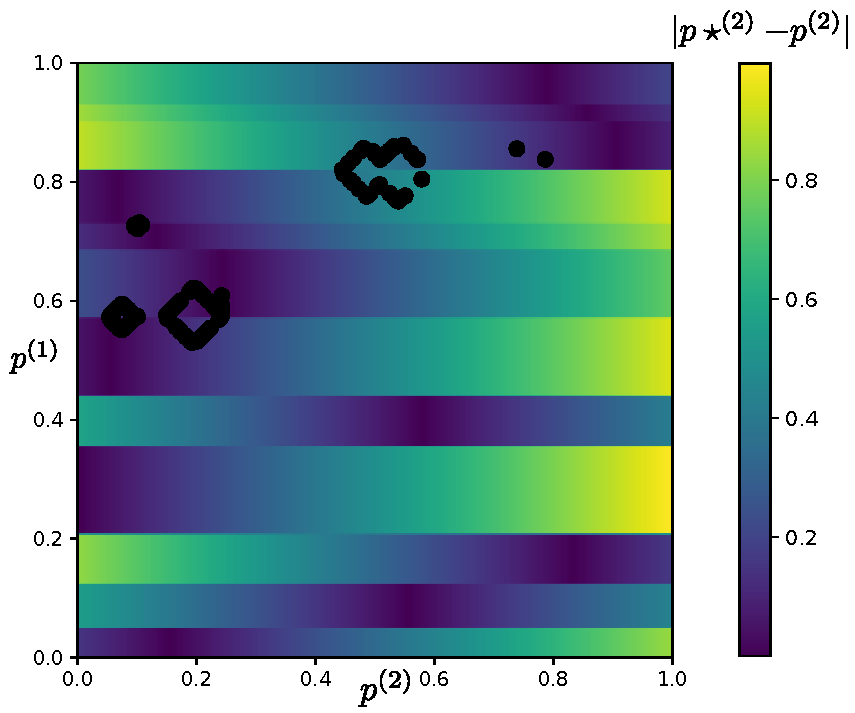
\includegraphics[width=\textwidth]{champ_Y_006_t1_notraj.pdf}
	\end{minipage}
	\caption{Valeur de $\lvert {\hat{p}}\m{1} - p\m{1} \rvert $, resp. $\lvert {\hat{p}}\m{2} - p\m{2} \rvert$ avant apprentissage, lorsque les poids sont disposés aléatoirement dans chaque carte.
	Les zones où ces valeurs sont nulles sont en violet sur le graphique. Les points fixes, s'il existent, sont aux positions de différence nulle pour $M\m{1}$ et $M\m{2}$, par exemple ici en $(0.1, 0.75)$.
	Les points noirs représentent les points d'arrivée de 200 trajectoires de relaxation, lancées pour différents $(\bmu_0\m{1}, \bmu_0\m{2})$.
	Ces tracés montrent que la valeur finale de la relaxation dépend ici des valeurs d'initialisation de la relaxation. Le BMU n'a donc pas de sens au début de l'apprentissage. \label{fig:diff_relax_t1_notraj}}
	\end{figure}

En figure \ref{fig:diff_relax_t1_notraj}, nous traçons les deux quantités $\lvert \hat{p}\m{1} - p\m{1} \rvert$ et $\lvert \hat{p}\m{2} - p\m{2}\rvert$ pour une configuration de poids prise avant l'apprentissage. Les poids sont alors disposés aléatoirement.
Les positions annulant chacune des quantités sont les zones en violet sur chaque graphique.
Nous y faisons figurer uniquement les positions de fin de relaxation des trajectoires $(\bmu\m{1},\bmu\m{2})$ pour plus de lisibilité. Ces valeurs finales sont marquées par les points noirs.

Nous remarquons une position située en $(0.1, 0.75)$, pour laquelle les deux champs s'annulent. Ce point fixe apparaît comme un hasard du choix des poids.
Nous observons des points noirs à cet emplacement, montrant que certaines trajectoires de relaxation ont bien évolué vers cette position. 
Cependant, d'autres trajectoires ont égalemement amené la suite $\mathbf{\bmu}_\tau$ vers d'autres positions finales.
Nous observons en particulier la présence de plusieurs cycles limites, par exemple autour des positions $(0.5, 0.8)$~: certaines trajectoires ne convergent pas et évoluent sur ce cycle de positions. Les points noirs observés sur le graphique correspondent dans ce cas aux dernières positions atteintes au temps $\tau_{max}$ de la relaxation.

Afin de représenter autrement les trajectoires, nous nous intéressons également en \ref{fig:champ_0} au champ des déplacements de $(\bmu\m{1}_\tau,\bmu\m{2}_\tau)$ lors de la relaxation, en fonction de la position courante. 
Nous y superposons les trajectoires complètes aboutissants aux points présentés en figure \ref{fig:diff_relax_t1_notraj}.
Ces champs de déplacement mettent en évidence les trajectoires de $(\mathbf{\bmu})_\tau$ qui mènent à un point fixe et celles qui mènent à des cycles limites.
Nous observons notamment que les cas de non-convergence sont uniquement des cycles limites~: nous n'observons pas de trajectoire ayant une évolution chaotique.

Cette observation montre qu'en début d'apprentissage, la relaxation n'a pas de sens en tant que recherche de BMU~: il existe certes un point fixe vers lequel certaines trajectoires ont convergé, mais les trajectoires restent dépendantes de l'initialisation de la relaxation. 
Elles ne sont donc pas relatives uniquement à la configuration des poids des cartes et à l'entrée externe.
Il est important de noter que malgré ces cas de non-convergence, les cartes évoluent quand-même vers un état organisé en fin d'apprentissage. Par ailleurs, ces cas de non-convergence sont ici seulement des cycles limites.

Cette observation renforce également l'intérêt d'initialiser la relaxation au maximum de l'activité externe et non aléatoirement dans l'espace des positions, afin de mieux contraindre l'évolution de la relaxation.

	\begin{figure}
		\centering
		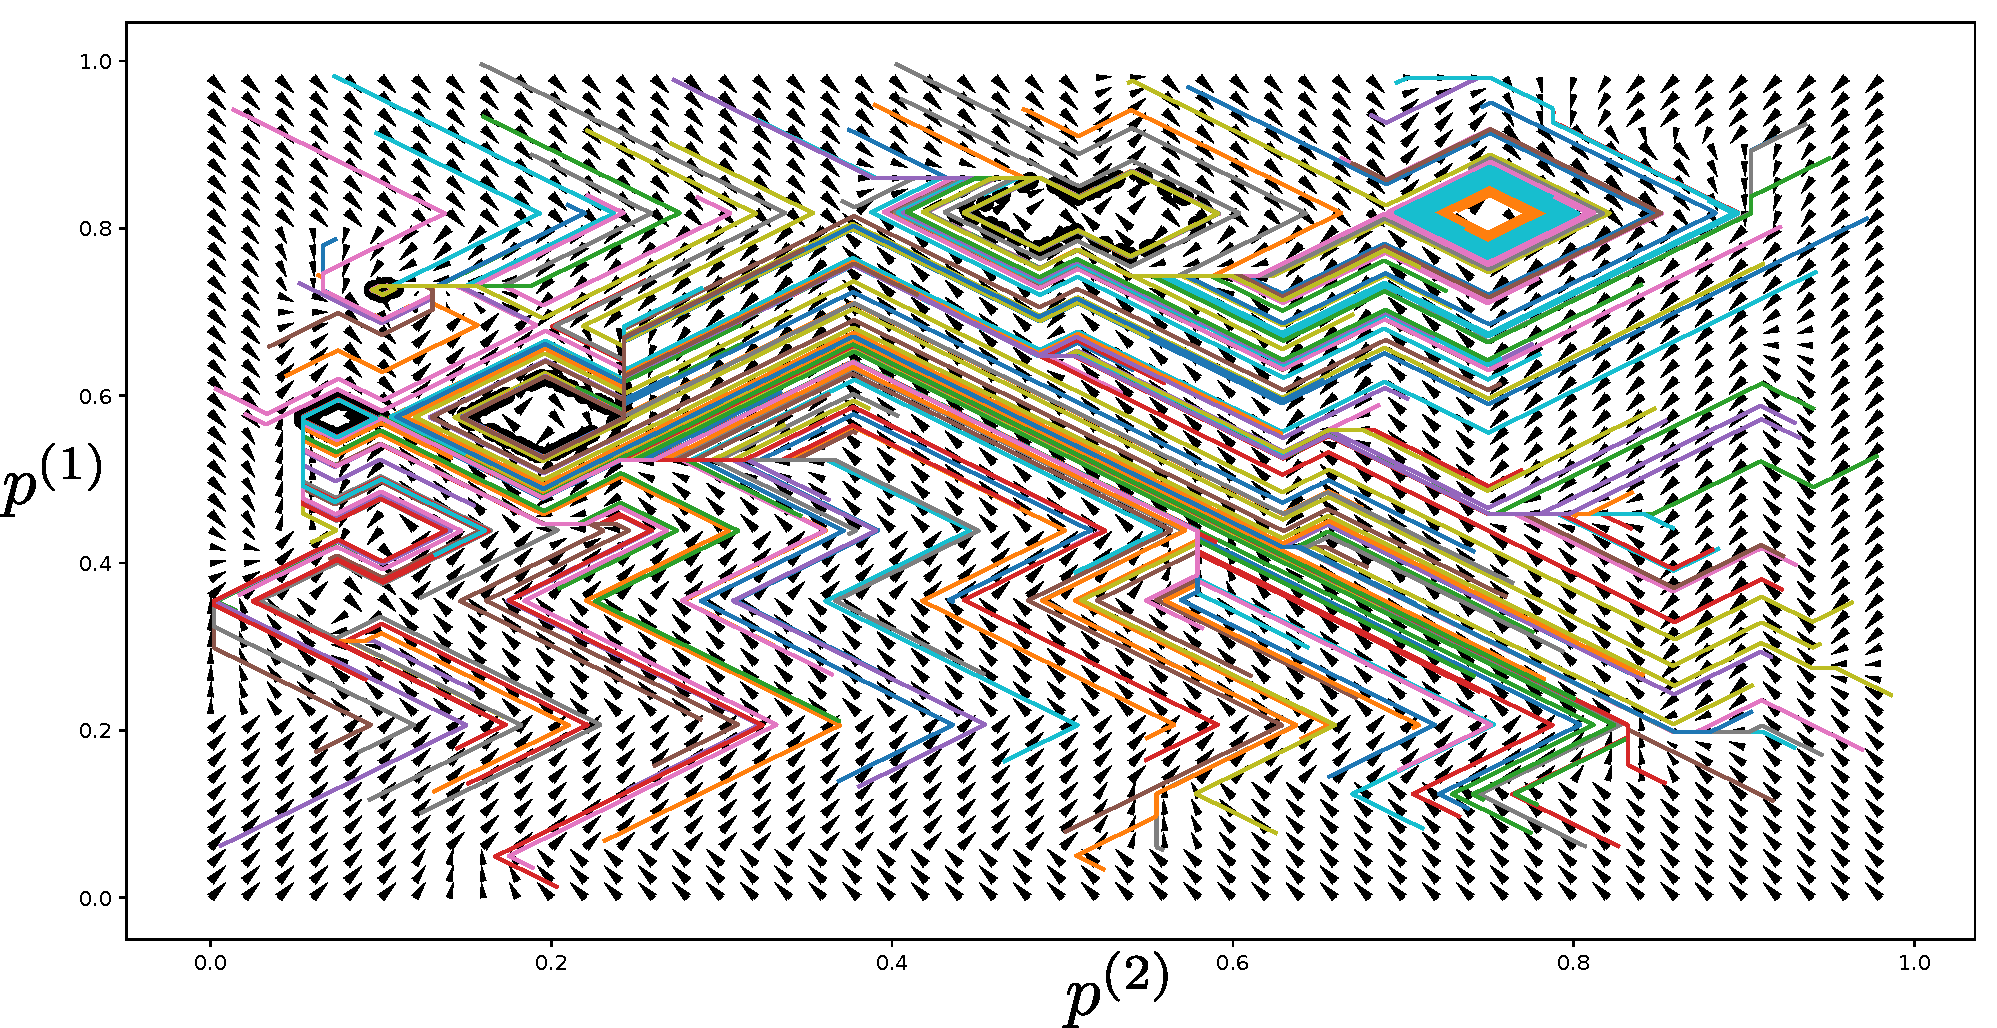
\includegraphics[width=\textwidth]{champ_006_t1.pdf}
		\caption{Champ des déplacements à effectuer de $(\bmu\m{1}_\tau, \bmu\m{2}_\tau)$ selon $(p\m{1}, p\m{2})$ lorsque les poids sont aléatoires, à $t=0$. Nous représentons les trajectoires de 200 relaxations initialisées différemment. Ces tracés mettent en valeur les comportements de cycles limites, observés autour des positions $(0.2, 0.6)$ ou $(0.5, 0.8)$.}
		\label{fig:champ_0}
		\end{figure}
		
\subsection{\'Evolution de la relaxation après dépliement des poids}
\begin{figure}
	\begin{minipage}{0.5\textwidth}
	\centering
	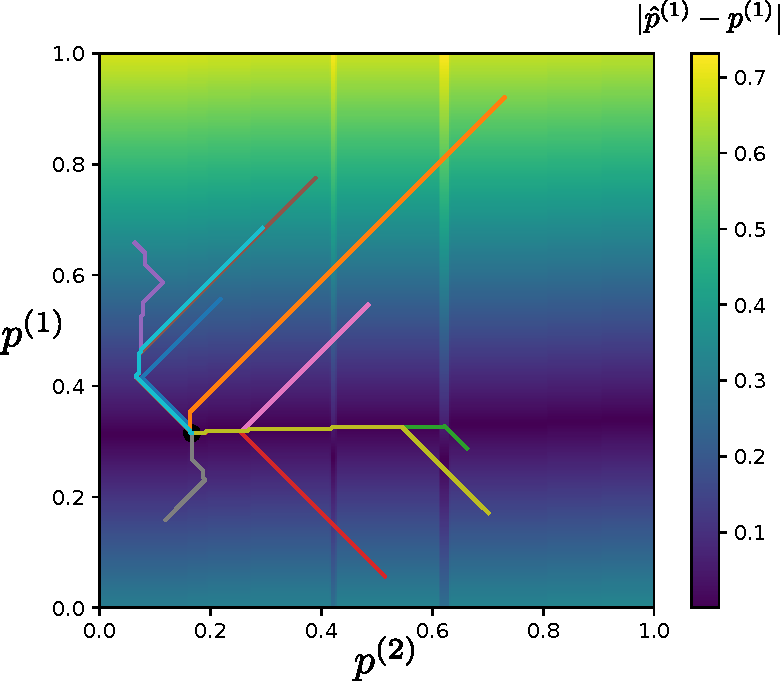
\includegraphics[width=\textwidth]{champ_X_006.pdf}
	\end{minipage}
	\begin{minipage}{0.5\textwidth}
	\centering
	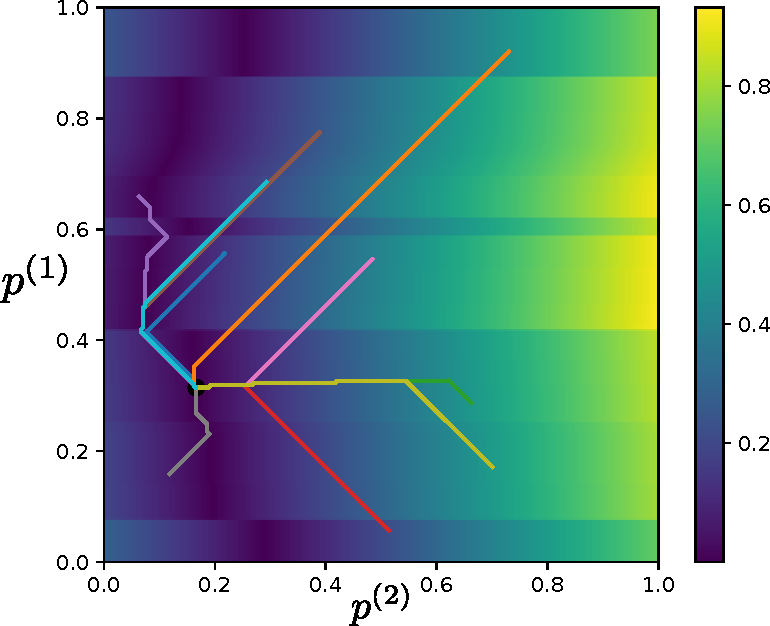
\includegraphics[width=\textwidth]{champ_Y_006.pdf}
	\end{minipage}
	\caption{Valeur de $\lvert{\hat{p}}\m{1} - p\m{1}\rvert$, resp. $\lvert{\hat{p}}\m{2} - p\m{2}\rvert$, lorsque les cartes sont organisées telles que représentées en figure \ref{fig:w006}. 
	Les points noirs représentent les points d'arrivée de la relaxation pour 200 trajectoires de relaxation, dont 10 d'entre elles sont tracées sur le graphique, lancées pour différents $(\bmu_0\m{1}, \bmu_0\m{2})$. Toutes ces trajectoires de relaxation convergent vers le même point, qui est l'unique point fixe de la fonction générant la suite $\mathbf{\bmu}_\tau$. Le BMU a donc un sens, car la relaxation ne dépend pas de l'initialisation du BMU.
	\label{fig:diff_relax_notraj}}
	\end{figure}

Nous nous intéressons maintenant à l'évolution de la relaxation dans une configuration de poids organisée, obtenue après une phase d'apprentissage d'une architecture de deux cartes.
La configuration de poids obtenue sur laquelle ont été réalisés les tracés est représentée en figure~\ref{fig:w006}. 
Les poids externes sont dépliés sur tout $[0,1]$, et les poids contextuels présentent également une continuité. Nous reviendrons sur la disposition particulière des poids contextuels dans les chapitres suivant~: nous notons seulement que les poids externes sont organisés de manière monotone, et que les poids contextuels sont organisés de manière monotone sur des sous-régions de cartes.

En figure~\ref{fig:diff_relax_notraj}, nous représentons les champs $\mathbf{g}$. 
Les tracés font apparaître une structure dans les valeurs des champs.
Un point unique où les deux différences sont nulles existe à l'intersection des deux zones violettes. Ce point est le seul point d'attraction toutes pour les trajectoires~: nous observons un seul point noir sur les tracés.
La figure \ref{fig:champ_9999} présente le champ de déplacement des BMUs en fonction de la position courante. 
Nous retrouvons l'évolution des trajectoires de relaxation vers cet unique point d'attraction. Nous remarquons que les trajectoires semblent suivre les régions où $\mathbf{g}$ est nul dans l'une ou l'autre des cartes, pour mener à la position stable. 

Sur cet exemple, la relaxation ne dépend donc plus des conditions initiales. La fonction $\mathbf{f}$ admet un unique point fixe. 
Le BMU a donc ici un sens pour l'apprentissage~: il ne dépend que des entrées externes et de l'état de la carte, et non du processus de relaxation. D'après l'équation $\ref{eq:opti}$, il s'agit d'une position maximisant l'activité totale des cartes de l'architecture.
Nous avons retrouvé ce même comportement sur des expériences sur plusieurs valeurs d'entrées et configurations de poids, que nous n'avons pas tracées ici.


\begin{figure}
\centering
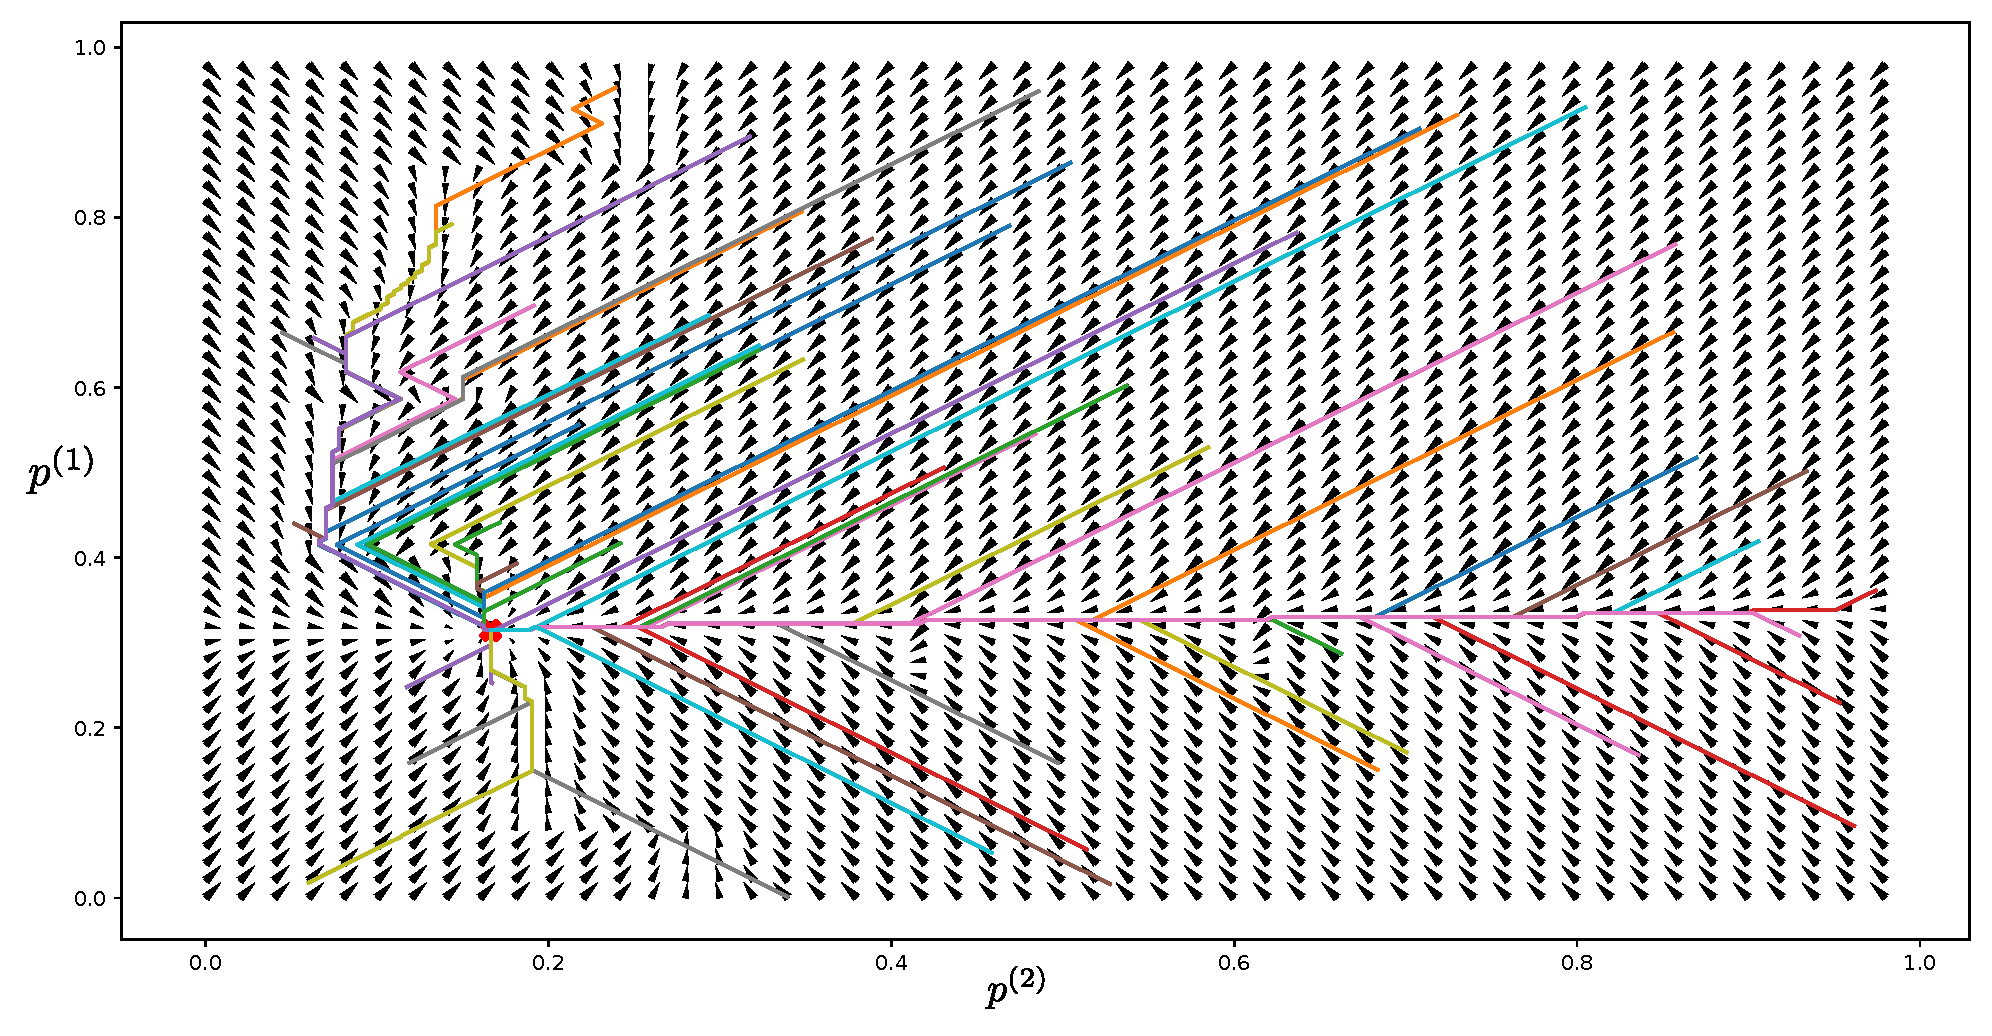
\includegraphics[width=\textwidth]{champ_006.pdf}
\caption{Champ des déplacements à effectuer de $(\bmu\m{1}_\tau, \bmu\m{2}_\tau)$ selon $(p\m{1}, p\m{2})$, calculé pour des poids organisés après apprentissage, représentés en figure \ref{fig:w006}. Nous y représentons les trajectoires suivis par 50 relaxations initialisées différemment. Les relaxations évoluent vers un point fixe commun.}
\label{fig:champ_9999}
\end{figure}

\subsection{Discussion}
La structure observée dans les champs $\mathbf{g}$ nous invite à supposer que l'existence de cet unique point de convergence vient de la disposition ordonnée des cartes en fin d'apprentissage. 
\`A la fin de l'apprentissage, les poids externes sont organisés de façon montone~: dans chaque carte, $a_e(\inpx,p)$ présente un seul pic d'activation.
De plus, l'activité contextuelle vient seulement moduler les valeurs de l'entrée externe, rendant l'influence de l'entrée contextuelle $\inpc$ sur la position du maximum d'activation moindre par rapport à l'influence de $\inpx$.
Nous illustrons cette influence en figure \ref{fig:w006}. 
Nous faisons figurer les poids des deux cartes après apprentissage à droite. 
\`A gauche, nous représentons les valeurs de $\hat{p}\m{1}$ et $\hat{p}\m{2}$, obtenues pour une même entrée externe $\mathbf{\inpx} = (0.26, 0.06)$ fixée, en faisant varier l'entrée $\inpc\m{1}$ sur toutes les positions de la carte $M\m{2}$, et inversement.
Quelle que soit l'entrée contextuelle $\inpc\m{1}$, nous remarquons que $\hat{p}\m{1}$ sera forcément situé entre $0.26$ et $0.34$.
Cette zone restreinte de la carte est indiquée en gris sur la figure de droite.
Ainsi, même si la relaxation ne convergeait pas, elle évoluerait forcément vers cette zone de la carte, dont les poids externes sont proches de l'entrée externe.

D'après cet exemple et les autres observations réalisées dans nos travaux, nous formulons l'hypothèse que le dépliement ordonné des poids externes dans une carte en 1D est une condition suffisante à l'existence d'un unique point fixe pour la suite $(\mathbf{\bmu})_\tau$, ou du moins à l'existence d'une région très réduite de la carte, autour du maximum de l'activité externe, fixant les limites d'évolution de $(\mathbf{\bmu})_\tau$.
Dans ce cas, la relaxation permettrait de se diriger vers cet unique point fixe ou cette zone.
Les BMUs trouvés par relaxation ont alors un sens pour l'apprentissage~: il correspondent à un point maximisant la somme des activités des cartes de l'architecture.
Une perspective d'étude de la relaxation pourrait donc être de démontrer expérimentalement ou analytiquement cette propriété. 
Toutefois, cette démonstration n'est pas un point clé de la construction de l'architecture CxSOM, dans la mesure où les observations que nous réaliserons dans la suite de cette thèse montrent qu'une architecture de cartes effectue un apprentissage des entrées, et ce malgré la non-convergence en début d'apprentissage. 
Le fait qu'un tel apprentissage soit rendu possible, malgré des cas de non-convergence de la relaxation, appuient expérimentalement l'utilisation de la relaxation comme méthode de connexions entre les cartes. 
De plus, nous avons présenté en section~\ref{sec:relax_conv} des indicateurs permettant de mesurer expérimentalement la convergence de la relaxation. Nous prendrons le soin de tracer ces indicateurs de convergence pour les différentes architectures que nous présenterons dans la suite de la thèse.


\begin{figure}
	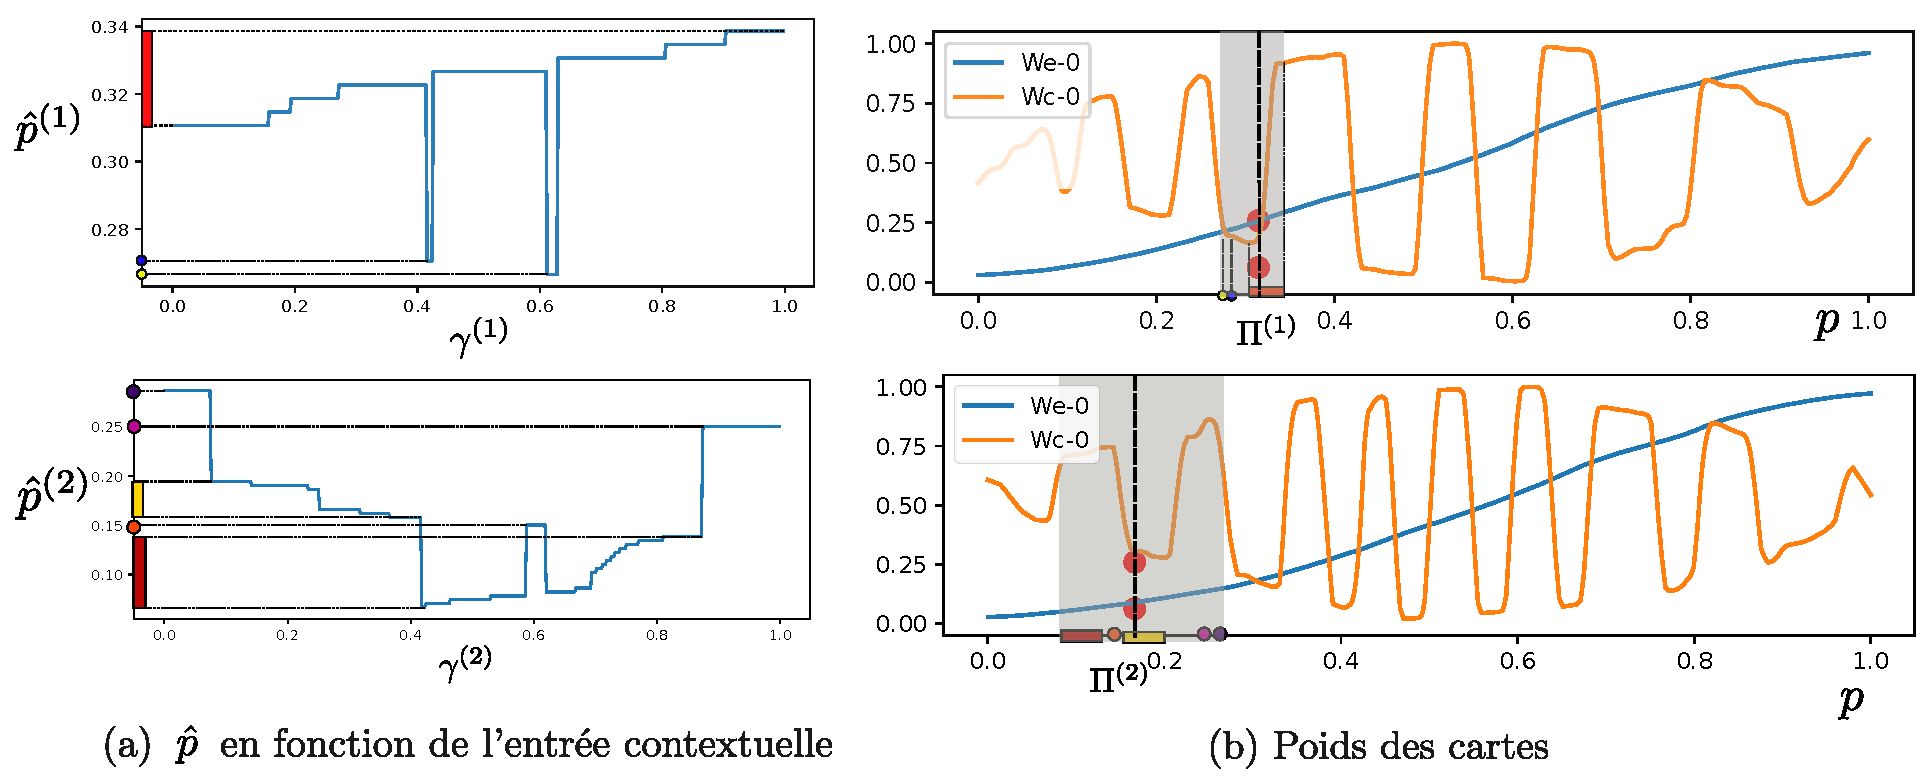
\includegraphics[width=\textwidth]{am_w_006_noinp}
	\caption{(a): $\hat{p}\m{1}$ et $\hat{p}\m{2}$ en fonction de l'entrée contextuelle de leur carte $\inpc\m{1}$ et $\inpc\m{2}$.(b): les poids externes et contextuels des cartes $1$ et $2$ sont représentés selon leur position dans la carte. On représente également les entrées test $\inpx\m{1}$ et $\inpx\m{2}$ en fonction de leur BMU. Les entrées utilisées pour tracer les figures de gauche sont colorées en rouge sur les figure de droite: $\inpx\m{1}=0.26,\inpx\m{2}=0.06$. Les intervalles dans lequel les valeurs de $\hat{p}$ varient sont grisés sur la figure (b)~ on observe que $\hat{p}$ reste dans une portion réduite de la carte, quelle que soit son entrée contextuelle.}
	\label{fig:w006}
	\end{figure}

% \subsection{Influence du pas de relaxation}

% Dans les expériences précédentes, nous avons utilisé un pas de déplacement $\Delta=0.05$.
% Une autre solution pour la relaxation est de ne pas utiliser $\Delta$, et, à chaque itération, déplacer le BMU $\bmu\m{i}_\tau$ directement en $\hat{p}\m{i}$.

% L'évolution de la relaxation devient alors:
% \begin{equation}
% \forall i, \bmu\m{i}_{\tau+1} = \hat{p}\m{i}_{\tau}
% \end{equation}

% On pourrait supposer que prendre un petit $\Delta$ permet une meilleure convergence; en fait, la valeur de $\Delta$ influence peu la capacité de convergence et l'organisation des cartes.
% En figure \ref{fig:diff_nopas}, nous avons tracé plusieurs trajectoires de relaxation réalisées après apprentissage sur une configuration de poids et une même entrée externe.
% Nous représentons sur cette même figure les différences $\lvert \hat{p}\m{1} - p\m{1} \rvert$ et $\lvert \hat{p}\m{2} - p\m{2} \rvert$.
% Le comportement de la relaxation ne change pas par rapport à celui observé en figure \ref{fig:diff_relax_notraj}~: les trajectoires tracées sur la figure convergent vers l'unique point pour lequel $\mathbf{p} = \mathbf{\hat{p}}$.
% Cela se comprend au vu des résultats précédents. $\hat{p}\m{1}$ et $\hat{p}\m{2}$ sont dans un intervalle réduit de valeurs de la carte, quelles que soient les positions $p\m{1}$ et $p\m{2}$. 
% Amener directement le BMU dans cet intervalle, ou l'y amener pas à pas avec $\Delta$, change peu l'évolution de la suite. 

% \begin{figure}
% \begin{minipage}{0.5\textwidth}
% 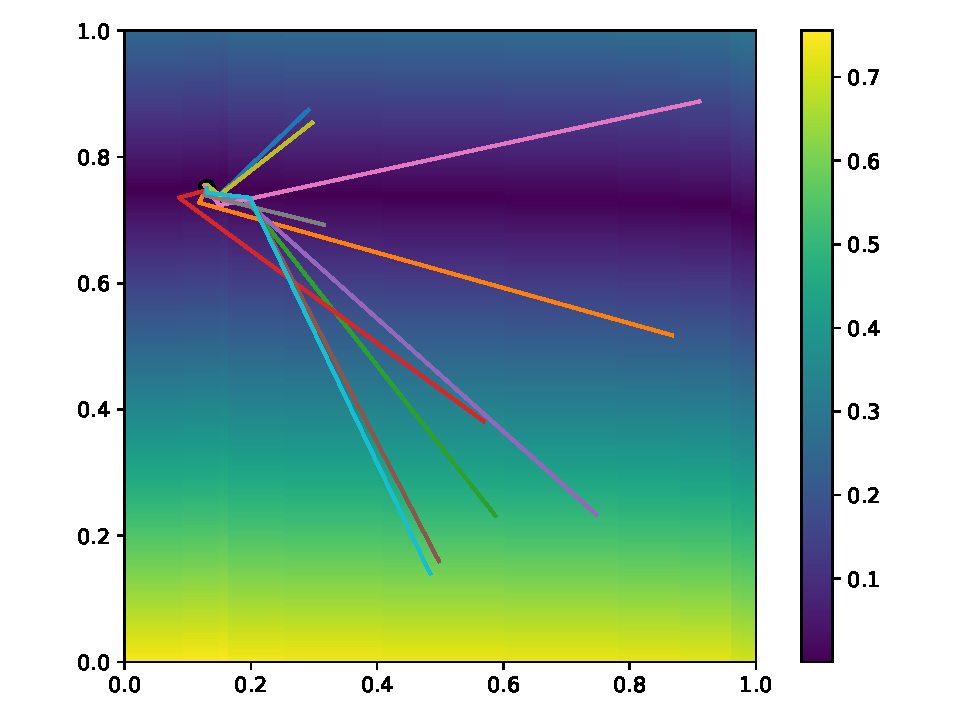
\includegraphics[width=\textwidth]{champ_X_009}
% \end{minipage}
% \begin{minipage}{0.5\textwidth}
% 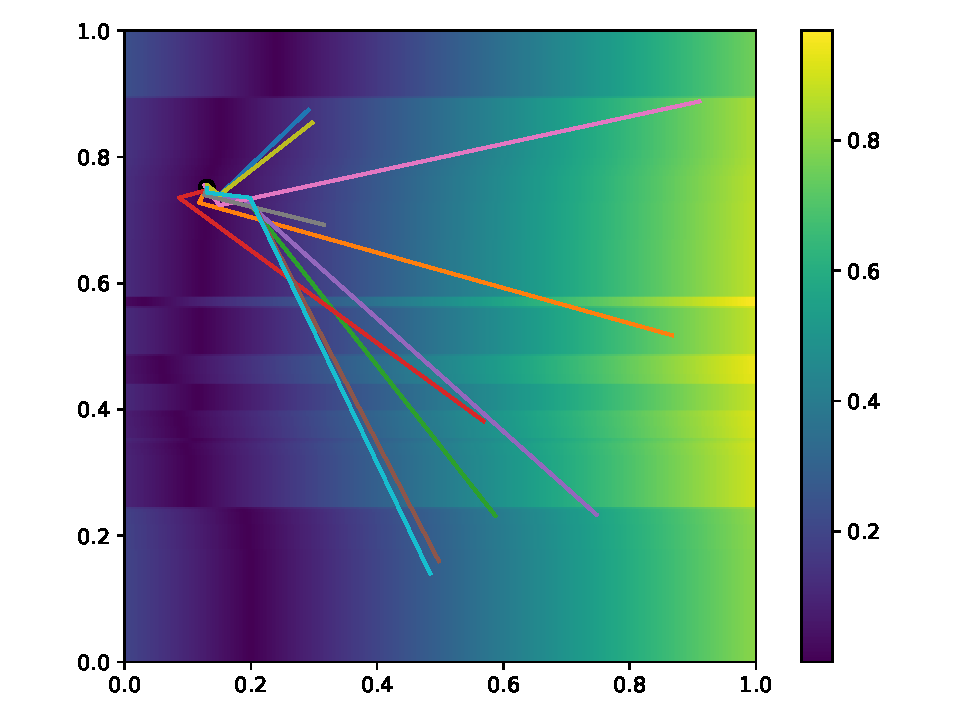
\includegraphics[width=\textwidth]{champ_Y_009}
% \end{minipage}
% \caption{Trajectoires des relaxations $(\bmu\m{1}_{\tau},\bmu\m{2}_\tau)$ dans le champ des différences $\lvert \hat{p}\m{1} - p\m{1} \rvert $ et $\lvert \hat{p}\m{2} - p\m{2} \rvert$, lorsque la relaxation est effectuée sans utiliser de petits déplacements. Les tracés sont effectués après apprentissage. La relaxation semble encore converger vers un point fixe.}
% \label{fig:diff_nopas}
% \end{figure}

% \section{Conclusion}

% Les parties \ref{sec:conv} et \ref{sec:cont} montrent donc que, lorsque les poids sont quelconques, la convergence de l'algorithme de relaxation n'est pas assurée; au contraire, la relaxation évolue dans la plupart des cas vers une situation non convergente. Dans le cas particulier étudié dans la section, il semble exister des point fixes, mais dus au caractère aléatoire des poids. La relaxation ne permet pas de trouver ces points. Pourtant, l'apprentissage des cartes utilisant la relaxation comme recherche de BMU mène une organisation des poids, même sans que la relaxation ne converge au début. Cette organisation permet de plus une meilleure convergence de la relaxation (convergence dans plus de $90 \%$ des cas).

% Ce comportement peut être expliqué. On observe que la relaxation converge bien à partir du moment où les poids externes sont organisés et présentent une continuité. 
% Au début de l'apprentissage, même si la relaxation mène à des positions quelconques de BMUs, ces BMUs auront quand même des poids externes restant proches de la valeur de l'entrée externe. 
% Le calcul de l'activité dépend en effet d'abord de l'activité externe de la carte:
% $$ a_g = \sqrt{a_e ( \beta a_e + (1-\beta a_c))}, \;\; \beta=0.5$$ 
% De plus, la relaxation est initialisée à une position correspondant au maximum de l'activité externe.

% L'organisation de la carte s'effectuera donc de façon similaire à une carte classique. Dans une carte de Kohonen, pour des poids aléatoires, de multiples positions de BMU sont possibles lors du calcul de la distance des poids à l'entrée. La disposition des poids et le choix du BMU n'influencent pas la propriété globale d'organisation d'une carte. Cette même observation peut s'effectuer ici. 
% Le rayon de voisinage externe étant bien plus grand que le rayon de voisinage contextuel, l'organisation des poids externes de la carte influence peu l'organisation des poids contextuels.
% Lorsque les poids externes présentent une continuité, la relaxation converge. Les poids contextuels peuvent alors s'organiser selon le BMU, qui a maintenant un sens: il s'agit d'un point fixe de la fonction de relaxation. Le BMU correspond alors au point qui maximise en même temps les activités globale de chaque carte.

% Expérimentalement, on observe que, lorsque les cartes sont organisés, le point fixe  existe, est unique est est atteint par n'importe quelle trajectoire de relaxation. Le BMU a donc un sens au niveau de la carte. 

% Enfin, la relaxation utilise un pas de déplacement utilisé $\delta$. 
%

% La relaxation est donc une recherche d'un maximum global à l'architecture, ce maximum étant un point fixe de la fonction de mise à jour des positions.
% Une fois que les poids externes d'une carte présentent une continuité, la relaxation et le BMU issu de ce processus ont un sens topologique: on observe expérimentalement que la fonction de mise à jour présente un point fixe $\mathbf{\bmu} = \mathbf{f}(\mathbf{\bmu})$, et que la relaxation converge vers ce point fixe. Ce point fixe est alors le point qui maximise \emph{collectivement} les activités globales de chaque carte de l'architecture.
% Bien que la relaxation ne converge pas au début de l'apprentissage, la convergence est observée dès que les poids externes présentent une certaine continuité. Cette continuité étant assurée après quelques itérations d'apprentissage par l'algorithme de mise à jours des poids de Kohonen, on peut donc dire que la relaxation converge au sein de CxSOM.


\section{Conclusion}

Ce chapitre a présenté des points d'analyse expérimentale de mécanisme de relaxation. 
Nous avons détaillé un formalisme décrivant l'algorithme de relaxation comme le déplacement des valeurs $\mathbf{\bmu}_\tau$ selon un champ $\mathbf{f}$ constant, qui dépend des configurations de poids de toutes les cartes ainsi que des entrées externes. 
Si la relaxation converge, elle converge vers les points fixes de ce champ. 
Ces points fixes s'expriment comme des solutions d'un problème d'optimisation global à l'architecture.
Nous avons conclu de la formalisation que si $\mathbf{f}$ admet un unique point fixe et que la relaxation converge, alors la valeur trouvée à l'issue de la relaxation correspond à la position maximisant la somme des activités globales de l'architecture.
Cette recherche de maximum est réalisée localement, au niveau de chaque carte, et non de façon globale. Ainsi, la relaxation agit comme une manière de connecter des cartes de façon non-hiérarchique en s'appuyant sur les BMUs comme interface. Il s'agit d'un processus dynamique hérité des DNF couplés, qui s'extrait des calculs gourmands et des nombreux paramètres des DNF pour proposer une dynamique simple et scalable à des architectures comportant de nombreuses cartes.

Nous avons proposé deux conditions pour que la relaxation puisse être considérée comme une recherche de BMU~: 
\begin{enumerate}
	\item nous attendons de la relaxation qu'elle converge,
	\item nous attendons que la valeur de convergence ne dépende pas de l'initialisation des trajectoires, rendant ainsi le BMU relatif aux entrées et poids des cartes et non au processus de recherche.
\end{enumerate}

Nous avons montré expérimentalement que la convergence de la relaxation dépend de la disposition des poids des cartes. Nous avons observé que lorsque les poids des cartes ne sont pas ordonnés, comme c'est le cas avant l'apprentissage, il n'existe pas forcément de solution au problème d'optimisation. 
Dans ce cas, la relaxation converge dans moins de 20\% des cas lors des étapes de test.
Pourtant, nous avons également observé que les cartes se déplient correctement, malgré l'instabilité de la relaxation en début d'apprentissage. Nous pensons que ce comportement est favorisé grâce à l'initialisation de la relaxation à des positions maximisant l'activité externe et grâce à la prépondérance de l'activité externe dans le calcul de l'activité globale. Nous avons par ailleurs observé sur les exemples que les cas de non-convergence semblent se traduire par des cycles limites sur des positions qui sont proches. 
Pour ces deux raisons, bien que la valeur trouvée à l'issue de la relaxation ne soit pas une solution du problème de maximisation globale, il s'agirait d'un point qui possède une valeur forte d'activité externe dans chaque carte~: $\w_e(\bmu)$ est proche de l'entrée externe $\inpx$. Cela permet aux poids externes de s'organiser correctement. Une fois que les poids externes sont dépliés, la relaxation apparaît converger.
Enfin, nous avons observé que lorsque tous les poids sont bien dépliés, il semble exister une solution unique maximisant les activités globales de chaque carte. L'algorithme de relaxation apparaît alors converger vers ce point quelles que soient les conditions initiales.
Lorsque les cartes sont organisées, le BMU obtenu à l'issue de la relaxation aurait donc bien un sens pour l'apprentissage~: il maximise la somme des activités des cartes, et ne dépend pas de l'initialisation de la relaxation.


Ces tracés de relaxation ont été effectués pour des cartes 1D prenant des entrées 1D, avec des cartes ayant un jeu de paramètres spécifique $r_e = 0.2$ et $r_c = 0.02$. Nous avons également observé que la relaxation converge sur des cartes 2D prenant des entrées 1D.
Dans les chapitre suivants, nous détaillerons le comportement des cartes 1D et 2D sur différentes données d'entrées et différents paramètres. Nous prendrons le soin de tracer dans ces chapitres l'évolution de la convergence de la relaxation, d'après la méthode proposée en figure~\ref{fig:conv_evolution}~; nous observerons que la relaxation semble converger dès que les poids présentent un dépliement ordonné, ceci sur des cartes 1D prenant des entrées 1D (chapitre~\ref{chap:analyse}), mais également sur des cartes 2D prenant des entrées 2D au chapitre~\ref{chap:analyse2D}.

\ifSubfilesClassLoaded{
    \printbibliography
    %\externaldocument{../main.tex}   
}{}
\end{document}
